\documentclass[oneside,12pt]{report}  

% the dimensions of the page
\textheight=9.25in \topmargin=-0.5in   %See note in Chapter 8 of Sample Report about "Page scaling" option in Adobe
\textwidth=6.0in
\oddsidemargin=0.3in
\evensidemargin=0.3in  % Needed to balance even and odd pages in twoside print copy


% Useful packages
\usepackage{dtklogos}
\usepackage [font=small, labelfont=bf]{caption}
\usepackage{amsmath}
\usepackage{bm}
%\usepackage[colorlinks=true,pagebackref,linkcolor=blue]{hyperref}
\usepackage{amsfonts}
\usepackage{amsthm}
\usepackage{amsmath}
\usepackage{algorithm}
\usepackage{algorithmic}
\usepackage{graphicx, subfigure}
\usepackage{caption}
\usepackage{excludeonly}
\usepackage{url}
\usepackage{graphicx} 

%\usepackage{doc}
%% Following sets up logic and formatting for conditional twoside copying
%\usepackage{ifthen, color, fancyvrb}
%\usepackage{nextpage}\pagestyle{plain}
%\newcommand\myclearpage{\cleartooddpage
%  [\thispagestyle{empty}]
%  }

\DeclareMathOperator*{\argmin}{arg\ min}
\DeclareMathOperator*{\sign}{sign}

% Note special alternative codes for using TWO bibliographies; see cautionary note in
\DeclareGraphicsExtensions{ps,eps,PNG,png}

% Theorem-like command definitions:
\newtheorem{theorem}{Theorem}[chapter]
\newtheorem{lemma}{Lemma}[chapter]
\newtheorem{definition}{Definition}  % Note, this italicizes everything

% Print the chapter and sections in the toc
\setcounter{tocdepth}{1}

% Specify which files to typeset for this run (note that overall pagination is preserved)
%\includeonly{chapter1, chapter2}
% Specify which files NOT to typeset for this run (note that overall pagination is preserved)
%\excludeonly{}

% Groundwork for allowing double-sided copying with blank versos
\def\prefacesection#1{
\chapter*{#1}
\addcontentsline{toc}{chapter}{#1}
}

\begin{document}


\def\thefootnote{\fnsymbol{footnote}}

\thispagestyle{empty}

% The numbers below controls the amount of space between the following sections
\def\shiftdowna{0.32in}  % Adjust for balance
\def\shiftdownb{0.22in}  % Adjust for balance

% Set up the boiler plate at the top of the page

\begin{center}
\textbf{{\large Mathematical Modeling and Consulting }}\\

\vspace \shiftdowna
%\includegraphics[width=0.5\textwidth]{jhu.png}\\

\includegraphics[width=2.5in]{BJU.jpg}\\

% Home Department
\vspace \shiftdowna
\underline {Sponsor}\\ 
\vspace{5pt}
\textbf{\large Blue Jays Unlimited} \\
\vspace\shiftdowna
\textbf{{Progress Report}}

% TITLE
\vspace \shiftdowna
\textbf{{\Large Modeling and Simulating Fan Participation at Large Scale Sporting Events}}

% STUDENTS
\vspace{0.35in}
\underline {Team Members}\\
\vspace{5pt}
Ahmed Aly, Department of Biomedical Engineering\\
\texttt{aaly2@jhu.edu} \\
\vspace{5pt}
Steven Su, Department of Biomedical Engineering\\
\texttt{ssu7@jhu.edu} \\
\vspace{5pt}
Danni Tang, Department of Biomedical Engineering\\
\texttt{danni@jhu.edu} \\
%\vspace{10pt}
%Jane Doe (Report Coordinator), Home Department
%%\texttt{jane.doe@jhu.edu}

% INSTRUCTOR
\vspace \shiftdownb
\underline {Academic Mentor} \\
\vspace{5pt}
\text{Dr.~N.~H.~Lee}, Applied Mathematics and Statistics\\
\texttt{nhlee@jhu.edu}

%% Consultants
%\vspace \shiftdownb 
%\underline {Consultant}\\
%\vspace{5pt}
%Jason Bourne\\

% DATE
\vspace \shiftdowna
Date: Last Compiled on \today

\end{center}

\vfill  %Fill page to force following note to bottom
\footnoterule
\noindent \small{This project is supported by Blue Jays Unlimited.}

% Begin ABSTRACT
\ifthenelse{\boolean{@twoside}}{\myclearpage}{}
\prefacesection{Abstract}
\paragraph{}
Having a loud and supportive home crowd is the ultimate home team advantage for any sports team. This is especially true for collegiate sports. In this work we developed a simple stochastic model for modeling cheering in crowds at large sporting events. Our model accounts for differences in innate support level for a sports team between fans as well as the number and length of time surrounding fans have been cheering. It uses these factors to predict whether a single fan will start to cheer and then simulates over time how cheering in a crowd progresses. The results from the model are promising: cheering in a crowd can either increase greatly or increase slightly, depending on how the parameters of the model are varied. 

% Begin ACKNOWLEDGMENTS
\ifthenelse{\boolean{@twoside}}{\myclearpage}{}
\prefacesection{Acknowledgments}
\paragraph{}
We would like to thank Blue Jays Unlimited for sponsoring us. In addition, we appreciate the unwavering support and patient guidance our academic mentor, Dr.~Nam H.~Lee, has given us. We would also like to thank our classmates for their support. 

% Table of contents, List of Figures, and List of Tables.
\ifthenelse{\boolean{@twoside}}{\myclearpage}{}
\tableofcontents

\ifthenelse{\boolean{@twoside}}{\myclearpage}{}
\listoffigures

%\ifthenelse{\boolean{@twoside}}{\myclearpage}{}
%\listoftables


\renewcommand{\thefootnote}{\arabic{footnote}}
\setcounter{footnote}{0}

\ifthenelse{\boolean{@twoside}}{\myclearpage}{}
\prefacesection{Introduction}
\paragraph{}
A loud and supportive home crowd is the ultimate home team advantage for any sports team. Past research has shown that the home crowd advantage can have a profound effect on deciding who wins a sporting event \cite{Jamieson_2010}. Across all major professional sporting leagues in the United States, the home team at any sporting event wins approximately 60\% of the time, a statistically significantly higher winning percentage then the expected 50\% \cite{Jamieson_2010}. The home crowd advantage is even more profound in college athletics. Studies have shown that in certain collegiate sports, the home team wins up to 66\% of the games played \cite{Snyder_1985}.

\paragraph{}
In addition to helping the home team win, a loud and supportive home crowd can also improve the ambiance of a sporting event. Whether fans are chanting the school fight song, waving a rally towel, doing the wave, or clapping in general applause, the fans are not only showing support for the home team but also enhancing the general atmosphere of the sporting event at the same time. Note that all of these actions will hence be collectively termed ``cheering.'' For this and previously stated reasons, it is evident that cheering is essential at collegiate sporting events. Cheering improves the collegiate sporting experience for both the athletic teams as well as the fans. 

\paragraph{}
The Johns Hopkins University, located in Baltimore, MD, has a proud athletic tradition to go along with its long standing reputation for strong academics. The Johns Hopkins University Blue Jays have amassed 47 national championships and 187 conference titles \cite{hopathletic}. The Blue Jays have excelled at many sports including Men's Lacrosse, Men's Swimming, Men's Football, and Men's Baseball. The Men's Lacrosse team has won 44 national championships, most recently in 2007, while the Men's Swimming team won 32 conference championships, including an astounding streak of 28 consecutive conference championships from 1971-1998 \cite{hopathletic}. More recently, the Men's Football and Baseball teams were each conference champions for three consecutive years from 2009 through 2011 \cite{hopathletic}. As with any collegiate athletic program, The Johns Hopkins University and its supporters are always looking for ways to improve its athletic teams' performances so that they may continue in their winning ways.

\ifthenelse{\boolean{@twoside}}{\myclearpage}{}
\prefacesection{Background}
\paragraph{} 
Blue Jays Unlimited (BJU), established in 1995, is a volunteer group of alumni, friends and staff dedicated to supporting and promoting Johns Hopkins athletics \cite{bjuwebsite}. BJU is the official booster club for Johns Hopkins athletics and has more than 3000 active members, who have raised more than \$4 million in funds to improve the Johns Hopkins athletic experience for both student athletes and fans alike \cite{bjuwebsite}. These funds provide money for capital projects as well as scholarship and operational endowments \cite{bjuwebsite}. Past BJU projects have included renovations of the Newton H.~White Athletic Center as well as recognition banners for championship teams \cite{bjuwebsite}.

\paragraph{}
BJU is present at nearly all major Johns Hopkins sporting events to encourage fans to support their Blue Jays in a vociferous and family-friendly manner to propel their Hopkins' teams to victory. It is their goal to provide Johns Hopkins' athletic teams with a spirited home crowd to cheer them on. As such, BJU is interested in maximizing the amount of fan participation in cheering at sporting events held on Homewood Field at the Homewood campus of The Johns Hopkins University. More specifically, they believe that they can increase fan participation in cheering events by strategically placing ``cheer starters'' in the home crowd to encourage other fans to participate in cheering. Cheer starters are student volunteers who lead and urge other fans around them to cheer.

\begin{figure}[h]
	\begin{center}
			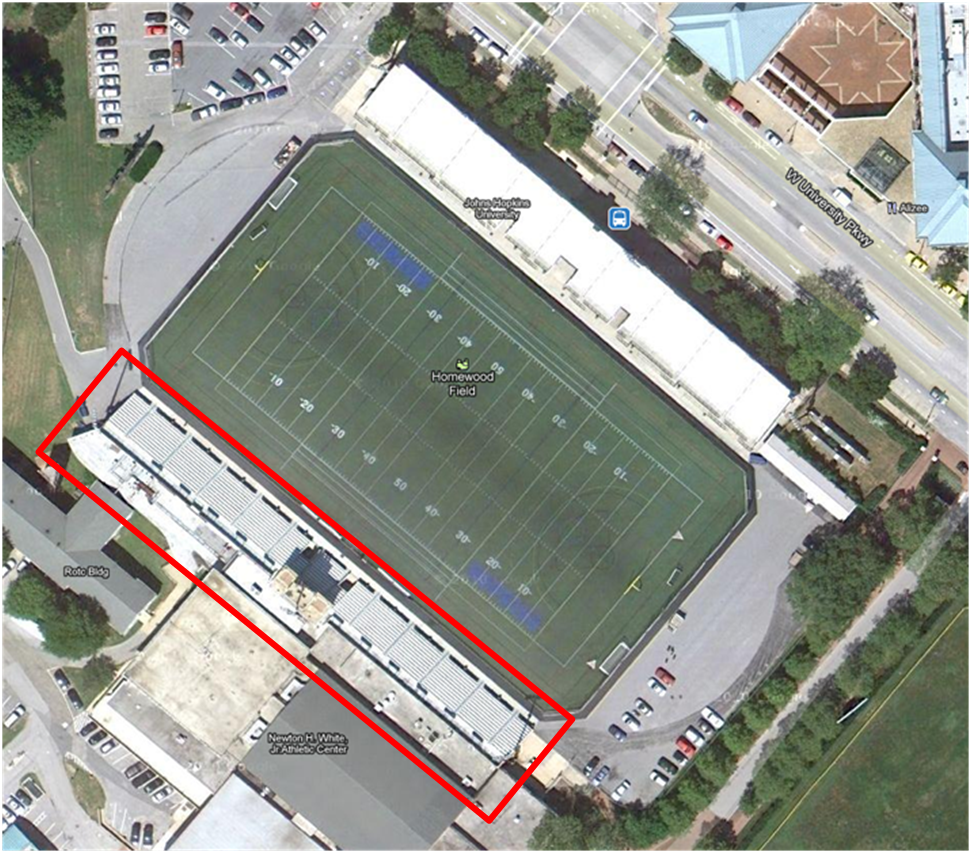
\includegraphics[height=2.25in] {Bleachers.png}
	\end{center}
	\caption[Homewood Field located on the Homewood campus of The Johns Hopkins University in Baltimore, MD.]{Homewood Field located on the Homewood campus of The Johns Hopkins University in Baltimore, MD. The bleachers in the lower left corner outlined in red are traditionally reserved for home team fans.}
	\label{fig:homewoodfield}
\end{figure}

\paragraph{}
Consider the satellite image of Homewood Field in Figure \ref{fig:homewoodfield}, courtesy of Google Maps. Homewood Field's capacity is approximately 8500 spectators \cite{wiki}. The long rectangular section of bleachers outlined in red in the lower left of portion of the image seats approximately 4000 fans and is traditionally reserved for Blue Jays' fans. For nearly all major Hopkins' sporting events, these home team bleachers are filled to capacity. As such, BJU is specifically interested in maximizing fan cheering in these home team bleachers. 

\ifthenelse{\boolean{@twoside}}{\myclearpage}{}
\prefacesection{Problem Statement and Objectives}
{\bf{\Large Problem Statement}}
\paragraph{}
BJU wants to know if cheer starters can actually increase cheering and also wants a simple model of fan participation in cheering in the home team bleachers on Homewood Field.
\newline
\newline
{\bf{\Large Objectives}}
\paragraph{}
Our task is to provide BJU with a simple model of fan participation in cheering at Homewood Field in the home team bleachers as well as simulation results from the model which determine if their belief about cheer starters is accurate. If cheer starters are found to be effective, we will attempt to provide BJU with more details about the quantity and location at which cheer starters should be placed in order to maximize cheering, time permitting.

\ifthenelse{\boolean{@twoside}}{\myclearpage}{}
\prefacesection{Analysis}
Because this model is a simulation, it is imperative to clearly define simplifications and assumptions we have made in the model.
\paragraph{Simplifications and Assumptions}
	\begin{itemize}
	\item The willingness of a fan in a crowd to cheer depends on the number of people cheering around the given fan as well as how long the surrounding people have been cheering. The greater the number of people surrounding a fan who are cheering, and the longer the surrounding people have been cheering, the more likely that fan will start to cheer.
	\item The innate support level a fan has for the team also influences the willingness of that fan to start cheering.
	\item Once a fan starts to cheer, he/she continues cheering until the end of the simulation.
	\item The performance of the sports team does NOT influence cheering.
	\end{itemize}

%\paragraph {Simplifications and Assumptions}
%
%The stimulus in this case would be the performance of the team. For the purpose of simplicity we will assume that the stimulus is average. From there, we can take a snap shot of the crowd's behavior and ignore the dependence of cheering on the team's performance. Each snap shot can be represented by a "round".  
%\newline
%For the internal state of the individual we can assign base "cheer number" using a stochastic process. We will simplify cheering as a probabilistic switch with a universal threshold that if exceeded the individual will be considered cheering otherwise the indivdual will not be cheering. This will simplify the problem because it will allow us to ignore the continuos gradient and different levels of cheering. 
%\newline
%We will simplify the relationship of the willingness to cheer and the surrounding individuals to only include the individuals that are directly surrounding the intended member.

\paragraph {Computational Simulation}
\paragraph{}
Using MATLAB, we start by generating an arbitrary sized $n$ x $m$ matrix, $X$, to represent a $nm$ sized crowd. The number of rows, $n$, and columns, $m$, can be changed based on the user's liking. However, for our purposes we are choosing to make $X$ a long rectangular matrix to imitate the physical dimensions of the home team bleachers on Homewood Field. The matrix $X$ represents a crowd and each element in it corresponds to a specific fan in the crowd. For example $X_{ij}$ represents fan $ij$. Each element in $X$ is filled with the corresponding fan's innate support level for the team. Each fan's innate support level was generated by sampling from a normal random distribution with a mean of 10 and a standard deviation of 1 as shown in (\ref{1}). 

\begin{equation}
X_{ij}\sim Norm(10,1),~\forall~i\in[1,n],~j\in[1,m]
\label{1}
\end{equation}

\paragraph{}
A normal distribution fits the distribution of innate support levels that a crowd of fans has very well. The majority of fans who attend sporting events are average or close to average fans; they will cheer if others around them cheer for a long enough time \cite{DI2003}. A smaller proportion are super fans who will cheer regardless of what anyone else around them is doing \cite{DI2003}. A smaller proportion of attendees may also be less supportive of the team; they require a greater amount of encouragement to start cheering than the average fan \cite{DI2003}. This is well represented in a normal distribution where most of the distribution is centered around the mean and an increasingly smaller proportion of the distribution is found moving away from the mean in both directions \cite{DI2003}. In this model the mean was set to 10 and the standard deviation was set to 1 to ensure that it was highly unlikely that a fan was assigned a negative innate support level. (i.e.~it is very unlikely to sample a number from the normal distribution that is more than 10 standard deviations from the mean.) This makes the math much easier when considering the dependence on the surrounding people, as it will be shown later.

\paragraph{}
Next, we set an initial threshold, $T_{init}$. The initial threshold is used to determine which of the fans in the matrix are \textit{initially} cheering. Another $n$ x $m$ matrix, $X'$, was then created. Each element in $X'$ is initially assigned a value of 1, if the corresponding element in $X$ (i.e.~the element in $X$ with the same row and column indices) had a value which was greater than or equal to the initial threshold, otherwise the element is given a value of 0. See (\ref{2}). $X'$ is the matrix used to keep track of who is cheering. A value of 1 in $X'$ means that given fan is cheering, while a value of 0 means that given fan is not cheering. 

\begin{equation}
X'_{ij}=1~if~X_{ij}\geq T_{init},~X'_{ij}=0~if~X_{ij}<T_{init}
\label{2}
\end{equation}

\paragraph{}
Any fan with an innate support level greater than 1 standard deviation above the mean is far above the average fan and can be considered a super fan who would be initially cheering. As such, $T_{init}$ was appropriately set to equal 11, which is 1 standard deviation above the mean of the normal distribution used to generate the innate support levels.

\paragraph{}
As previously stated, whether a fan starts to cheer depends on how many directly adjacent fans around the given fan are cheering, as well as the length of time those fans have been cheering. $S$ is a $n$ x $m$ matrix which stores how many people surrounding a given fan are cheering at a given time. Each element in $S$ has corresponding elements with the same row and column indices in both $X$ and $X'$, all of which store different model values for the same individual fan. We define a round, $r$, to be the passing of an arbitrary time interval (approximately 3-5 seconds, in this case). We then create a fourth $n$ x $m$ matrix, $Y$, and compute the individual elements of $Y$ according to (\ref{3}). 

\begin{equation}
Y_{ij}=X_{ij}(S_{ij})+r,~\forall~i\in[1,n],~j\in[1,m]
\label{3}
\end{equation}

Again, each element in $Y$ represents an individual fan and has corresponding elements in $X$, $X'$, and $S$, with the same row and column indices. We then compare each of the elements in $Y$ to an absolute threshold, $T_{absolute}$. If an individual's score in $Y$ is greater than or equal to the absolute threshold, the individual will begin to cheer, and we set the corresponding element in $X'$ equal to 1. This is shown in (\ref{4}). If the individual's score in $Y$ is less than the absolute threshold, we do nothing to the corresponding element in $X'$ (i.e.~it remains 0).  

\begin{equation}
X'_{ij}=1~if~Y_{ij}\geq T_{absolute}
\label{4}
\end{equation}

\paragraph{}
We repeat this process for each round (i.e.~compute $Y$, update $X'$ based on the new $Y$, and then update $S$ for the next round based on the new $X'$) until we reach the desired number of rounds, $R$. During each round, we take snapshots of the crowds by storing $X'$ for that round. By doing so, we can compare $X'$ between the rounds and also compute the percentage of fans who are cheering in each round. It is important to note, by computing $Y$ as shown in (\ref{3}), the likelihood of a fan starting to cheer increases with the number of surrounding fans who are cheering (i.e.~as $S_{ij}$ increases) and also increases with the length of time those fans have been cheering (i.e.~as $r$ increases).

\paragraph{}
The final output is a pictorial representation of of the cheering behavior over $R$ rounds as well as the percentage of fans who were cheering in each round.

\ifthenelse{\boolean{@twoside}}{\myclearpage}{}
\prefacesection{Results}

\begin{figure}[h]
    \begin{center}
        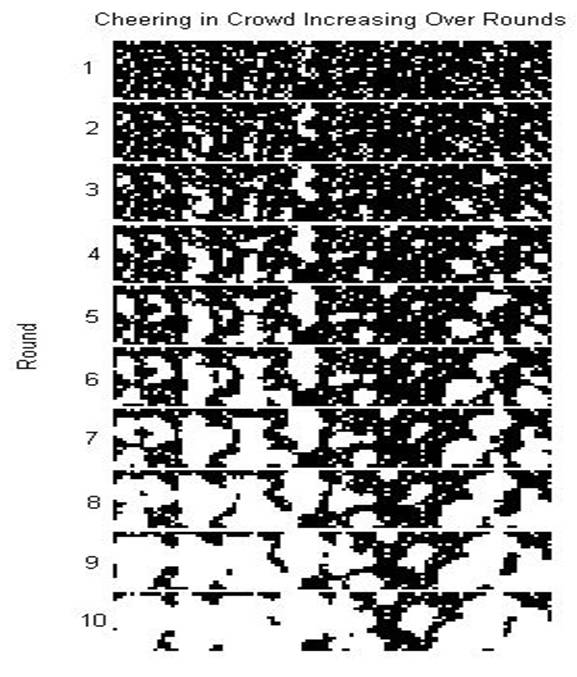
\includegraphics[height=2.5in]{sample_graph.jpg}
    \end{center}
    \caption[Pictorial representation of the progression of cheering over time with a lower absolute threshold.]{Pictorial representation of cheering in a 20 x 100 crowd for 10 rounds when $T_{absolute}=45$. White lines separate the results of each round. White represents the fans who are cheering and black represents fans who are not cheering.}
    \label{fig:graph1}
\end{figure}

\begin{figure}[h]
    \begin{center}
        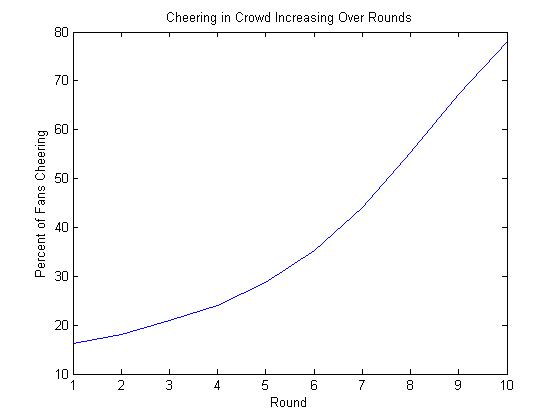
\includegraphics[width=3in]{sample_graph2.jpg}
    \end{center}
    \caption[Plot of cheering levels over time in a simulated crowd with a lower absolute threshold.]{The final percentage of cheering fans after each round are plotted when $T_{absolute}=45$.  An increase in the overall percentage of people cheering can be seen as the rounds progress.}
    \label{fig:graph2}
\end{figure}

\paragraph{}
Figure \ref{fig:graph1} and Figure \ref{fig:graph2} were generated by running our simulations with the following parameters: $n=20$, $m=100$, $T_{init}=11$, $T_{absolute}=45$, and $R=10$ rounds. As can be seen in Figure \ref{fig:graph1} and Figure \ref{fig:graph2}, our model predicts that as the rounds progress, more and more fans will begin to cheer. 

\begin{figure}[h]
    \begin{center}
        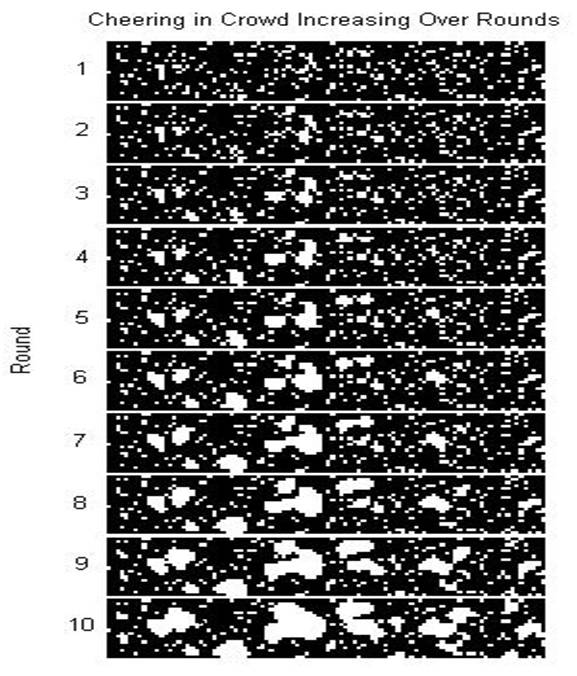
\includegraphics[height=2.5in]{sample_graph3.jpg}
    \end{center}
    \caption[Pictorial representation of the progression of cheering over time with a higher absolute threshold.]{Pictorial representation of cheering in a 20 x 100 crowd for 10 rounds when $T_{absolute}=50$. White lines separate the results of each round. White represents the fans who are cheering and black represents fans who are not cheering.}
    \label{fig:graph3}
\end{figure}

\begin{figure}[h]
    \begin{center}
        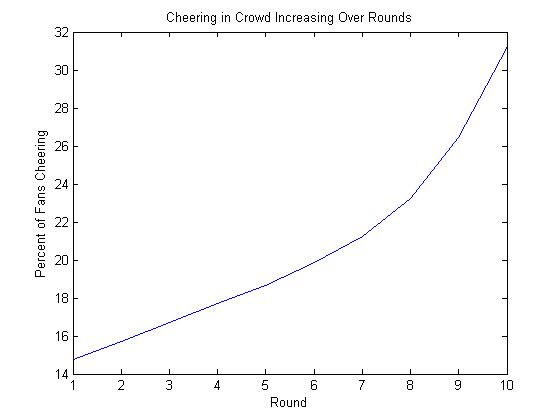
\includegraphics[width=3in]{sample_graph4.jpg}
    \end{center}
    \caption[Plot of cheering levels over time in a simulated crowd with a higher absolute threshold.]{The final percentage of cheering fans after each round are plotted when $T_{absolute}=50$. An increase in the overall percentage of people cheering can be seen as the rounds progress. However the increase is less than when a lower absolute threshold is used.}
    \label{fig:graph4}
\end{figure}

\paragraph{}
Figure \ref{fig:graph3} and Figure \ref{fig:graph4} were generated by running our simulations with all the parameters set the same as in Figure \ref{fig:graph1} and Figure \ref{fig:graph2} except that $T_{absolute}$ was set to 50. It is clear that by increasing $T_{absolute}$, the overall percentage of fans who end up cheering after 10 rounds decreases. This makes sense since a higher absolute threshold value will be harder to reach, and thus less fans will exceed the threshold and start cheering. 

\ifthenelse{\boolean{@twoside}}{\myclearpage}{}
\prefacesection{Remaining Work to Be Done}
\paragraph{}
For our current model, we picked sample parameters for purposes of demonstration so far. For example, our initial threshold is 11 (one standard deviation above the normal distribution centered at 10), and the absolute threshold was 45 or 50. The simulation ran for 10 rounds for a crowd of 2,000 people ($20$ x $100$ sized matrices). However, we have not yet determined an finalized set of model parameters for the entire project. For the remaining time we have to work on this project, we must pick a definitive initial threshold, absolute threshold, size of the crowd (i.e.~$n$ and $m$), and number of total rounds.
\paragraph{}
We must also investigate the effect of cheer starters on the percentage of fans cheering in the final round. Our current model does not take into account cheer starters; rather, it simulates a stochastic, general crowd susceptible to the influence of people cheering around them. Once all the parameters are finalized (including the number of cheer starters), we plan to randomly place the cheer starters within the crowd. We can then use Monte Carlo simulations to repeatedly run our model to determine the average percentage of fans cheering at the end of the final round when there are no cheer starters and also the percentage when there are cheer starters randomly placed in the crowd. If the final cheering percentage is statistically significantly greater with cheer starters then without, it would demonstrate that cheer starters are effective in increasing cheering. 
 
\paragraph{}
If time permits, we could also add a function to our model which allows us to manually dictate where the cheer starters are placed. This would allow us to try and find patterns in cheer starter placements which maximize cheering. Right now, we hypothesize certain patterns will produce a larger percentage of overall people cheering than other patterns.

\paragraph{}
Finally, we can complete the project by polishing the code in MATLAB and writing R documentation for a MATLAB coded-R documented package. We will also need to write a final report and give a final presentation.
%\include{D_Analysis}
%\include{E_Results}
%\include{F_Conclusion}

%\include{chapter1}
%\include{chapter2}
%\include{chapter3}
%\include{chapter4}
%\include{chapter5}
%\include{chapter6}


\appendix
\ifthenelse{\boolean{@twoside}}{\myclearpage}{}
\prefacesection{Glossary}

%\chapter{Lemmas}\label{Lemma}

%\chapter{Glossary}\label{Glossary}

%\vspace{12pt} 

\vspace{8pt} \noindent {\bf Cheering}. Any action performed by a fan which shows support for a sports team. Examples include chanting the school fight song, waving a rally towel, doing the wave, or clapping in general applause.

\vspace{8pt}
\noindent {\bf Cheer Starter}. A student volunteer who leads and urges other fans around him/her to cheer.


\ifthenelse{\boolean{@twoside}}{\myclearpage}{}
\prefacesection{Abbreviations}
%\chapter{Abbreviations}\label{Abbreviations}


\noindent {\bf BJU}.  Blue Jays Unlimited

%\vspace{5pt}
%
%\noindent {\bf JHU.}  Johns Hopkins University

%\endinput

% Add your bibliography to Contents
\ifthenelse{\boolean{@twoside}}{\myclearpage}{\newpage}
\addtocontents {toc}{\protect \contentsline {chapter}{REFERENCES}{}}
\addcontentsline{toc}{chapter}{Selected Bibliography Including Cited Works}  

% Bibliography must come last.
\bibliographystyle{unsrt}
\renewcommand\bibname{Selected Bibliography Including Cited Works}
%\nocite{*}  % List ALL references in your references, not just the ones cited in the text.
% This scheme automatically alphabetizes the Bibliography.
\bibliography{biblioWS}
\end{document}
